"The fundamental decision of investing is the allocation of your assets: How much should you own in stock? How much should you own in bonds? How much should you own in cash reserves"

\begin{multicols}{2}
    
\subsection{Expected Value}
Suppose that a return $R_i$ on asset i is equal to $R_i(s)$ in state s. And that states'
probabilities of occurrence are given by p(s), for s = 1, ..., S.
\begin{gather*}
    E[R_i] = \sum_{s=1}^{S}R_i(s)p(s)
\end{gather*}

\subsection{Variance}
The volatility or risk of $R_i$ is often refer to the \textbf{standard deviation} $\sigma_i$ (will be redefined later)
\begin{gather*}
    \begin{split}
        Var[R_i] &= \sigma_i^2 = E[(R_i(s)-E[R_i])^2]\\
        &= \sum_{s=1}^{S}p(s)(R_i(s)-E[R_i])^2
    \end{split}
\end{gather*}

\subsection{Covariance}
The degree of two assets in a portfolio move in the same direction at the same time.
\begin{gather*}
    Cov(R_i,R_j) = \sum_{s=1}^{S}p(s)(R_i(s)-E[R_i])(R_j(s)-E[R_j])\\
    Var[wA+vB] = w^2Var[A]+v^2Var[B] + 2wvCov[A,B]
\end{gather*}

\subsection{Correlation}
Measure the strength and direction two assets in a portfolio moves at the same time. 
\begin{gather*}
    Corr(R_i,R_j) = \rho_{ij}=\frac{Cov(R_i,R_j)}{\sigma_i\sigma_j}
\end{gather*}

\subsection{Portfolio Allocation}
\subsubsection{1 risky, 1 risk-free}
\underline{\textbf{Risk-free asset:}}\\
A baseline to compare with risky assets. normally deemed as the US Treasury Bill (not true this year). 
\begin{gather*}
    E[R_f] = R_f,\hspace*{0.3cm}V[R_f] = 0,\hspace*{0.3cm}Cov[R_f] = 0
\end{gather*}
The expected return for this kind of portfolio can be express as,
\begin{gather*}
    \begin{split}
        E[R_p] &= E[wR_i+(1-w)R_f]\\
        &= \boxed{R_f+w\overbrace{E[\underbrace{R_i-R_f}_\text{excess return}]}^\text{risk premium}}
    \end{split}
\end{gather*}
and the variance of the portfolio will be 
\begin{gather*}
    \begin{split}
       V[R_p] &= V[wR_i+(1-w)R_f]= w^2\sigma_i^2\\
        \sigma_p &= \lvert w\rvert\sigma_i
    \end{split}
\end{gather*}
\underline{\textbf{The Captial allocation line:}}\\
substituting the above, we can re-express expected value as the following, this is also know as the Capital Allocation Line, where the only possible combination of 1 risky and 1 risk-free lies on this line. What the investor \textit{can} get.
\begin{gather*}
    E[R_p] = R_f+wE[R_i-R_f] = R_f+\underbrace{\frac{E[R_i-R_f]}{\sigma_i}}_\text{Sharpe ratio}\sigma_p
\end{gather*}
\underline{\textbf{Indifference Curve:}}\\
Indifference curves expresses sets of portfolios that would make investors equally happy, they must slope upwards, and it also increases value from left to right. Indifference curves represent what investors want. If risk-neutral, Indifference curves becomes straight lines.

\underline{\textbf{Utility Function:}}\\
uses mean-variance utility to measure how risk tolerant and risk averse investor will value stocks
\begin{gather*}
    E[U(R_p)] = E(R_p)-0.5A\cdot V(R_p)
\end{gather*}
$A$ is a measure of risk aversion, the bigger the A is, the more risk averse the investor is. 

\subsubsection{2 risky, 1 risk-free}
\begin{figure}[H]
    \centering
    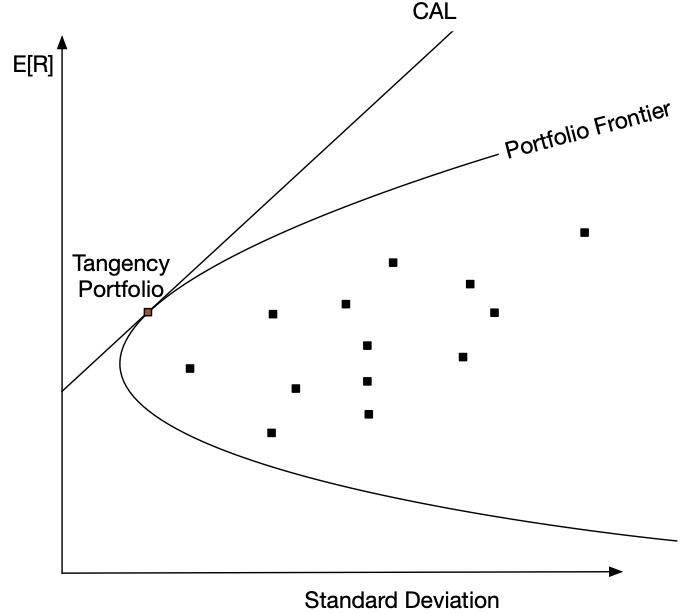
\includegraphics[width =0.3\textwidth]{Figure/cal.png}
\end{figure}
\subsubsection{Equal-Weighted Portfolio}
Equally weighted portfolio of independent assets. $Cov(R_i,R_j)=0$, variance of the portfolio then becomes, 
\begin{gather*}
    \sigma_p^2 = \frac{1}{N}\sum_{i=1}^{N}\sigma_i^2 = \frac{1}{N}E[\sigma_i^2]
\end{gather*}
Risk decreases with the number of assets. Standard deviation declines with the number of assets.


\end{multicols}